
%%%
%%% CHAPTER
%%%
\chapter{Global Optimisation Methods}\label{Chapter:GlobalOpt}


%%%
%%% Section
%%%
\section{Introduction}\label{Chapter:GlobalOpt:Section:Introduction}

%%% Subsection
\subsection{Main Definitions}\label{Chapter:GlobalOpt:Section:Definitions}
The main aim of optimisation methods is to find the {\it global optimum} (maximum or minimum) of a function. \citet{Pardalos_2000} \citep[see also][]{Piro_2016} gives a good overview on global optimisation methods. However, global optimum are often difficult to obtain except in a few problems. 

\begin{itemize}
%%%
\item {\bf Constrained and Non-Constrained Problems:} A \underline{constrained minimisation problem} is defined as,\index{Optimisation!Constrained problems}\index{Optimisation! Non-Constrained problems}
\begin{shaded}
   Given an {\it objective function} $f\left(\cdot\right):\mathcal{S}\subset\mathcal{R}^{n}\rightarrow\mathcal{R}$, where $\mathcal{S}$ is either the constraints or the solutions set of the optimisation problem $\mathcal{P}$,
\begin{displaymath}
   \mathcal{P}: \text{ Minimise }\; f(x)\; \text{ such that }\; x\in\mathcal{S}, 
\end{displaymath}
where $x=\left(x_{1},\cdots,x_{n}\right)$.
\end{shaded}

However, if $\mathcal{S}=\mathcal{R}^{n}$ then the problem is called  \underline{non-constrained minimisation problem}, i.e., the objective function $f$ must be minimised without explicit constraints,
\begin{shaded}
   Given an {\it objective function} $f\left(\cdot\right):\mathcal{S}\subseteq\mathcal{R}^{n}\rightarrow\mathcal{R}$, where $\mathcal{S}$ is either the constraints or the solutions set of the optimisation problem $\mathcal{P}$.
\begin{displaymath}
    \mathcal{P}: \text{ Minimise }\; f(x)\; \text{ such that }\; x\in\mathcal{R}^{n}. 
\end{displaymath}
where $x=\left(x_{1},\cdots,x_{n}\right)$.
\end{shaded}

%%%
\item {\bf Conditions for Optimality:}\index{Optimisation! Conditions for optimality} Indeed, for such problems we need to obtain first- and second-order necessary and sufficient conditions for optimality, defined by the following theorems\footnote{Proof of these theorems and definitions can be found in any advanced linear algebra and optimisation text books.}:

%%% Theorem:
\begin{thm}[First-Order Optimality Conditions]\label{Chapter:GlobalOpt:TheoremFirstOrder}
Let $f:\mathcal{R}^{n}\rightarrow\mathcal{R}$ be differentiable at a solution coordinate $x^{\ast}\in\mathcal{R}^{n}$. If $x^{\ast}$ is a local solution of problem $\mathcal{P}$, then $\nabla f\left(x^{\ast}\right)=0$.
\end{thm}

%%% Theorem:
\begin{thm}[Second-Order Optimality Conditions]\label{Chapter:GlobalOpt:TheoremSecondOrder}
Let $f:\mathcal{R}^{n}\rightarrow\mathcal{R}$ be twice differentiable at a solution coordinate $x^{\ast}\in\mathcal{R}^{n}$. 
   \begin{enumerate}
       \item If $x^{\ast}$ is a local solution of problem $\mathcal{P}$, then $\nabla f\left(x^{\ast}\right)=0$ and $\nabla^{2}f\left(x^{\ast}\right)$ is positive semi-definite (necessary condition).
       \item If $\nabla f\left(x^{\ast}\right)=0$ and $\nabla^{2}f\left(x^{\ast}\right)$ is positive definite, then there is an $\alpha > 0$ such that $f\left(x\right)\ge f\left(x^{\ast}\right)+\alpha\left\|x+\alpha\right\|^{2}$ for all $x$ near $x^{\ast}$ (sufficient condition).
   \end{enumerate}
\end{thm}

%%%
\item {\bf Convex Functions:} Theorem~\ref{Chapter:GlobalOpt:TheoremSecondOrder} establishes both 2$^{\text{nd}}$-order necessary and sufficient conditions for a problem whereas Theorem~\ref{Chapter:GlobalOpt:TheoremFirstOrder} describes 1$^{\text{st}}$-order necessary conditions. The sufficiency conditions is given by the following definition:

%%% Definition:
\begin{defn}[Convex Sets and Functions] For
   \begin{enumerate}
       \item A subset $\mathcal{C}\subset\mathcal{R}^{n}$ is assumed convex if for every pair $x$ and $y$ taken from $\mathcal{C}$, the entire line segment connecting $x$ and $y$ is also contained in $\mathcal{C}$,
           \begin{displaymath}
              \left[x,y\right]\subset\mathcal{C}\;\;\;\text{ where }\;\;\; \left[x,y\right]=\left\{\left(1-\lambda\right)x +\lambda y : 0\le\lambda\le 1\right\}
           \end{displaymath}
       \item A function $f:\mathcal{R}^{n}\rightarrow \mathcal{R}\cup\left\{\pm\infty\right\}$ is assumed convex if the set\footnote{The {\it epigraph (epi)} of a function $f:X\rightarrow\left[-\infty,+\infty\right]$ is the subset of $\mathcal{R}^{n}$ given by,
            \begin{displaymath}
                \text{epi}(f) = \left\{\left(x,w\right)\left|\; x\in X,w\in\mathcal{R}, f(x) \le w\right.\right\}.
            \end{displaymath}
          The {\it effective domain (dom)} of the function $f$ is the set
            \begin{displaymath}
                \text{dom}(f) = \left\{x\in X \left|\; f(x) < \infty\right.\right\}.
            \end{displaymath}
           } 
           \begin{displaymath}
              \text{epi}(f) = \left\{\left(\mu,x\right): f(x)\le \mu\right\}
           \end{displaymath}
           is a convex subset of $\mathcal{R}^{n+1}$. We can also define the set 
           \begin{displaymath}
              \text{dom}(f) = \left\{x\in\mathcal{R}^{n} : f(x) < +\infty\right\}
           \end{displaymath}
   \end{enumerate}
\end{defn}

%%% Lemma:
\begin{lem}
    The function $f : \mathcal{R}^{n}\rightarrow\mathcal{R}$ is convex \underline{if and only if} for every two solution coordinates, $\left\{x_{1},x_{2}\right\}\in\text{ dom}(f)$ and $\lambda\in\left[0,1\right]$ there is
       \begin{displaymath}
          f\left(\lambda x_{1} +\left(1-\lambda\right)x_{2}\right) \le \lambda f\left(x_{1}\right) + \left(1 - \lambda\right)f\left(x_{2}\right),
       \end{displaymath}
i.e., the secant line connecting $\left(x_{1},f\left(x_{1}\right)\right)$ and $\left(x_{2},f\left(x_{2}\right)\right)$ lies above the graph of $f$.
\end{lem}


%%% Theorem:
\begin{thm}\label{Theorem_Convex1}
   Let $f:\mathcal{R}^{n}\rightarrow\mathcal{R}\cup\left\{\pm\infty\right\}$ be convex. If $x^{\ast}\in\text{dom}(f)$ is a local solution to problem $\mathcal{P}$, then $x^{\ast}$ is a global solution to the problem $\mathcal{P}$.
\end{thm}

If $f$ is a differentiable convex function then a better solution can be obtained, thus this solution can be obtained from the following lemma.
%%% Lemma:
\begin{lem}\label{Lemma_Convex}
    Let $f : \mathcal{R}^{n}\rightarrow\mathcal{R}\cup\left\{+\infty\right\}$ be convex:
       \begin{enumerate}
          \item Given  $x\in\text{ dom}(f)$ and $d\in\mathcal{R}^{n}$, the ratio
             \begin{displaymath}
                 \frc{f(x+td)-f(x)}{t}
             \end{displaymath}
             is a monotonically increasing function of $t\in\left(0,+\infty\right)$.
          \item For every $x\in\text{ dom}(f)$ and $d\in\mathcal{R}^{n}$, the directive derivative $f^{\prime}\left(x;d\right)$ always exist and is given by
             \begin{displaymath}
                 f^{\prime}\left(x;d\right) = \displaystyle\inf_{t>0} \frc{f(x+td)-f(x)}{t}.
             \end{displaymath}
          \item For every $x\in\text{ dom}(f)$, the function $f^{\prime}\left(x;\cdot\right)$ is positively homogeneous,
             \begin{displaymath}
                 f^{\prime}\left(x;\alpha d\right) = \alpha f^{\prime}\left(x;d\right) \hspace{.5cm} \forall d\in\mathcal{R}^{n},\; \alpha > 0,
             \end{displaymath}
              and subadditive,
             \begin{displaymath}
                 f^{\prime}\left(x;u+v\right) \le f^{\prime}\left(x;u\right) + f^{\prime}\left(x;v\right).
             \end{displaymath}
       \end{enumerate}
\end{lem}

%%%
\item {\bf Differentiable Function and Local and Global Minima:} From {\it Lemma}~\ref{Lemma_Convex},
%%% Theorem:
\begin{thm}\label{Theorem_Convex2}
   Let $f:\mathcal{R}^{n}\rightarrow\mathcal{R}\cup\left\{+\infty\right\}$ be convex and also let's suppose that $x^{\ast}\in\mathcal{R}^{n}$ is a solution coordinate at which $f$ is differentiable. Then $x^{\ast}$ is a global solution to the problem $\mathcal{P}$ if and only if $\nabla f\left(x^{\ast}\right)=0$.
\end{thm}

%%% Theorem:
\begin{thm}\label{Theorem_Convex3}
   Let $f:\mathcal{R}^{n}\rightarrow\mathcal{R}$:
     \begin{enumerate}
        \item If $f$ is differentiable on $\mathcal{R}^{n}$, then the following statements are equivalent:
             \begin{enumerate}
                 \item $f$ is convex;
                 \item $f(y)\ge f(x)+\nabla f(x)^{\text{T}}\left(y-x\right)$ for all $[x,y]\in\mathcal{R}^{n}$;
                 \item $\left(\nabla f(x)-\nabla f(y)\right)^{\text{T}}(x-y) \ge 0$ for all $[x,y]\in\mathcal{R}^{n}$;
             \end{enumerate}
        \item If $f$ is twice differentiable then$f$ is convex if and only if $f$ is positive semi-definite for all $x\in\mathcal{R}^{n}$.
     \end{enumerate}
\end{thm}

This establishes that $f^{\prime}\left(x;d\right)$ exists for all $x\in\text{ dom}(f)$ and $d\in\mathcal{R}^{n}$. For a brief discussion of the continuity properties of this function is available in the following lemma:
%%% Lemma:
\begin{lem}
    Let $f:\mathcal{R}^{n}\rightarrow\mathcal{R}\cup\left\{+\infty\right\}$ be convex. Then, $f$ is bounded in a neighbourhood of a solution coordinate $x^{\ast}$ if and only if $f$ is Lipschitz\footnote{
Let $f:\mathcal{R}^{n}\rightarrow\mathcal{R}^{n}$, the Lipschitz-continuous function is defined by:
    \begin{enumerate}[(a)]
       \item Given an open set $\mathcal{B}\subseteq\mathcal{R}^{n}$, a function $f$ is called Lipschitz-continuous on the open subset $\mathcal{B}$ is there is a constant $\Lambda\in\mathcal{R}_{0}^{+}$ such that,
           \begin{displaymath}
               \left\|f(x)-f(y)\right\| \le  \Lambda\left\|x-y\right\|, \hspace{.5cm} \forall[x,y]\in\mathcal{B}.
           \end{displaymath}
       \item The function $f$ is called locally Lipschitz-continuous, if for each $z\in\mathcal{R}^{n}$ there is an $L>0$ such that $f$ is Lipschitz-continuous on the open sphere of center $z$ and radius $L$,
           \begin{displaymath}
              \mathcal{B}_{L}(z) = \left\{y\in\mathcal{R}^{n} :\left\|y-z\right\| < L\right\}.
           \end{displaymath}
       \item If $f$ is Lipschitz-continuous on all $\mathcal{R}^{n}$ space $\left(\text{i.e., }\mathcal{B}=\mathcal{R}^{n}\text{ in (a) above}\right)$, then $f$ is called globally Lipschitz-continuous.

    \end{enumerate}}
 in a neighbourhood of $x^{\ast}$.
\end{lem}

%%% Definition:
\begin{defn}[Local Minima]
   A solution coordinate $x^{\ast}$ is a local solution of a problem if there is a neighbourhood 
   \begin{displaymath}
           \Omega\left(x^{\ast},\Omega\right) = \left\{ z \left|\;\;\left|z-x^{\ast}\right| < \delta ; \delta > 0\right.\right\},
   \end{displaymath}
   such that $f\left(x^{\ast}\right)\leq f\left(x\right)\;\;\forall x\in\Omega\left(x^{\ast},\Omega\right) \cap \mathcal{S}$.
\end{defn}

%%% Definition:
\begin{defn}[Global Minima]
   A solution coordinate $x^{\ast}\in\mathcal{S}$ is a global solution of a problem if $f\left(x^{\ast}\right)\leq f\left(x\right)\;\;\forall x\in\mathcal{S}$.
\end{defn}

%%%
\item {\bf Convergence Conditions:} Optimisation methods are often based on iterative methods, in which after an initial solution $\left(\text{or estimate}, x^{\circ}\right)$ is chosen, a sequence of points $\left\{x^{k}\right\}$ is obtained through a prescribed algorithm. The sequence must converge to the solution $x^{\ast}$ of the problem.
%%% Definition:
\begin{defn}[Local Covergence]
   An algorithm is locally convergent if there is a positive scalar $\sigma$ such that for any initial solution coordinate $x^{\circ}\in\mathcal{R}^{n}$ $\left(\text{or } x^{\circ}\in\mathcal{S}\right)$, with $\left|x^{\circ}-x^{\ast}\right|\leq\sigma$, the algorithm generates a sequence of solutions that converges to the solution $x^{\ast}$.
\end{defn}

%%% Definition:
\begin{defn}[Global Covergence]
   An iterative algorithm is globally convergent if for any initial solution coordinate $x^{\circ}\in\mathcal{R}^{n}$ $\left(\text{or } x^{\circ}\in\mathcal{S}\right)$, the algorithm generates a sequence of solutions that converges to the solution $x^{\ast}$.
\end{defn}

\bigskip
Convergence is assumed asymptotic if the solution is not found after a finite number of iterations. Generally, globally convergent algorithms change search directions at each new coordinate, $x^{k}$. Therefore,

%%% Definition:
\begin{defn}[Descendant Direction] A linearly independent vector $d\in\mathcal{R}^{n}$ represents a descendant direction of a real function $f$ in $x\in\mathcal{R}^{n}$ if there is $\delta>0$, such that $f\left(x+t d\right)<f\left(x\right)$ for any $t\in\left.\left(0,\delta\right.\right]$.   
\end{defn}

%%% Definition:
\begin{defn}[Feasible Direction] A linearly independent vector $d\in\mathcal{R}^{n}$ represents a feasible direction of a real function $f$ in $x\in\mathcal{S}$ if there is $\theta >0$, such that $x+t d\in \mathcal{S}$ for all $t\in\left.\left(0,\theta\right.\right]$.   
\end{defn}

\end{itemize}

%%% Subsection
\subsection{Conditions of Optimality}\label{Chapter:GlobalOpt:Section:ConditionsOptimality}
Let $f:\mathcal{R}^{n}\rightarrow\mathcal{R}$ with $x^{\ast}$ be a global extremum (minimum or maximum) of the function.

%%% Subsection
\subsubsection{Non-Constrained Optimisation}
  \begin{enumerate}[{\bf i)}]
      \item {\bf First-Order Condition (necessary):} If $x^{\ast}$ is the extremum (i.e., maximum or minimum) of a function $f$, then this function is differentiable in $x^{\ast}$. Thus a necessary condition is,
          \begin{displaymath}
             \nabla f\left(x^{\ast}\right) = 0.
          \end{displaymath}
      \item  {\bf Second-Order Condition (necessary):} If $x^{\ast}$ is the local extremum (i.e., maximum or minimum) of a function $f$, then it is necessary that the function be twice differentiable in $x^{\ast}$, i.e.,
          \begin{displaymath}
             \nabla f\left(x^{\ast}\right) = 0.
          \end{displaymath}
and the Hessian matrix $\mathcal{H}\left(x^{\ast}\right)$,
          \begin{displaymath}
             \mathcal{H}\left(x^{\ast}\right) \equiv \nabla^{2} f\left(x^{\ast}\right) \text{ is positive (minimum) / negative (maximum) semi-definite}.\index{Hessian matrix ! Conditions of optimality}
          \end{displaymath}
      \item {\bf Sufficient Condition:} Let's $f(x)$ be a function twice differentiable in $x^{\ast}$ such that,
          \begin{eqnarray}
             &&\nabla f\left(x^{\ast}\right) = 0, \nonumber \\
             && \text{and } \mathcal{H}\left(x^{\ast}\right) \text{ is positive (minimum) / negative (maximum) definite,} \nonumber 
          \end{eqnarray}
           thus $x^{\ast}$ is a strict local extremum of function $f$.
  \end{enumerate}

The Hessian matrix, $\mathcal{H}\left(x^{\ast}\right)$, can be assessed through,
\begin{enumerate}[(a)]
   \item Contribution of the second-order term of the Taylor expansion around $x^{\ast}$,
         \begin{displaymath}
            f(x) - f\left(x^{\ast}\right) = \frc{1}{2}\left(x-x^{\ast}\right)^{\text{T}} \mathcal{H}\left(x^{\ast}\right)\left(x-x^{\ast}\right) + \cdots
         \end{displaymath}
   \item Eigenvalues (characteristic values) signs of $\mathcal{H}\left(x^{\ast}\right)$,
         \begin{displaymath}
            \mathcal{H}\left(x^{\ast}\right) = V \Lambda V^{-1},
         \end{displaymath}
         where $V$ and $\Lambda$ are matrices of eigenvectors (columns) and eigenvalues (diagonals), respectively. As the Hessian matrix is symmetric $\left(\text{and therefore }V^{-1}=V^{\text{T}}, \text{i.e., orthogonal matrix}\right)$ and defining $z(x)=V^{-1}\left(x-x^{\ast}\right)$, thus $\left(x-x^{\ast}\right)^{\text{T}}V=z^{\text{T}}$. Then the Taylor expansion around $x^{\ast}$ can be expressed as
         \begin{displaymath}
            f(x) - f\left(x^{\ast}\right) = \frc{1}{2}z^{\text{T}}\Lambda z + \cdots = \frc{1}{2}\summation_{i=1}^{n}\lambda_{i}z_{i}^{2} + \cdots,
         \end{displaymath}
         where $\lambda_{1},\cdots,\lambda_{n}$ are the determinants of {\it principal minors} of the matrix $\Lambda$.
   \item Determinant signs of the main {\it principal minors} of $\mathcal{H}\left(x^{\ast}\right)$ (Sylvester criterion). Below,  we summarise the relationship between $\mathcal{H}\left(x^{\ast}\right)$ and its first principal minor of order $k$, $\mathcal{M}_{k}\left(\mathcal{H}\right)$,
    \begin{center}
        \begin{tabular}{|c | c c c|}
           \hline
              {\bf $\mathcal{H}\left(x^{\ast}\right)$} & {\bf Taylor}  &  {\bf $\lambda$} & {\bf $\Delta_{k}=\text{det}\left(\mathcal{M}_{k}\right)$} \\
           \hline
             positive semi-definite & $x^{\text{T}}\mathcal{H}x \ge 0$ & $\ge 0$ &   $\ge 0$ \\
             positive definite      & $x^{\text{T}}\mathcal{H}x   > 0$ & $>   0$ &   $>   0$ \\
             negative semi-definite & $x^{\text{T}}\mathcal{H}x \le 0$ & $\le 0$ &   $(-1)^{k}\Delta_{k}\ge 0$ \\
             negative definite      & $x^{\text{T}}\mathcal{H}x   < 0$ & $<   0$ &   $(-1)^{k}\Delta_{k} > 0$ \\
             indefinite             & $x^{\text{T}}\mathcal{H}x (>/<) 0$& $(>/<) 0$ &   different from above \\
          \hline
        \end{tabular}
 %      \caption{Analysis of the Hessian matrix.}
    \end{center}
$\mathcal{M}_{k}\left(\mathcal{H}\right)$ is obtained from the removal of the last $n-k$ columns and rows of the matrix $\mathcal{H}$,
\end{enumerate}

Therefore,  we can say that $x^{\ast}$ is,
     \begin{itemize}
         \item Local minimum if $\mathcal{H}\left(x^{\ast}\right)$ is positive definite, $f(x) > f\left(x^{\ast}\right)$;
         \item Local maximum if $\mathcal{H}\left(x^{\ast}\right)$ is negative definite, $f(x) < f\left(x^{\ast}\right)$;
         \item Saddle point if $\mathcal{H}\left(x^{\ast}\right)$ is indefinite, thus eventually $f(x) < f\left(x^{\ast}\right)$ and $f(x) > f\left(x^{\ast}\right)$;
     \end{itemize}
     If $\mathcal{H}\left(x^{\ast}\right)$ is semi-definite then we need to further investigate high-order terms of the Taylor expansion.

%%% Subsection
\subsubsection{Constrained Optimisation}
Let $\mathcal{P}$ be an optimisation problem of function $f:\mathcal{R}^{n}\rightarrow\mathcal{R}$ subject to equality $\left[h(x)\right]$ and inequality $\left[g(x)\right]$ constraints,
    \begin{eqnarray}
        \mathcal{P}: \text{Minimise } f(x) && \nonumber \\
        \text{subject to}:&& h_{j}(x) = 0, \;\; j=1, \cdots, m \nonumber \\
                          && g_{j}(x) \le 0, \;\; j=1, \cdots, p \nonumber \\
                          && x\in X\subseteq \mathcal{R}^{n}, \nonumber 
    \end{eqnarray}
where $f(x)$, $g(x)$ and $h(x)$ $\in\mathcal{C}^{2}$. The set of all feasible points is defined as,
    \begin{displaymath}
        \mathcal{K} = \left\{x\in X\subseteq \mathcal{R}^{n}\; \left| \; h(x) = 0,\; g(x) \le 0\right. \right\}
    \end{displaymath}

An inequality constraint $g_{j}(x)$ is said to be {\it active} in a feasible point $\hat{x}$, if $g_{j}\left(\hat{x}\right)=0$, otherwise it is an {\it inactive constraint}. Active constraints impose a boundary in the viability region, whereas inactive constraints do not prescribe any boundary in the neighbourhood of point $\hat{x}$, which is defined by the hyper-sphere of radius $\varepsilon$ around this point, $\mathcal{B}_{\varepsilon}\left(\hat{x}\right)$. A vector $d$ is called {\it feasible directional vector} from the point $\hat{x}$, if there exist an hyper-sphere of radius $\varepsilon$ such that,
   \begin{displaymath}
      \left(\hat{x}+\lambda d\right) \in \left\{\mathcal{B}_{\varepsilon}\left(\hat{x}\right)\cap\mathcal{K}\right\}\;\;\forall \; 0\le \lambda\le \frc{\varepsilon}{\left|\ d\right\|}.
   \end{displaymath}
The set of vectors of feasible directions from $\hat{x}$ is commonly called{\it cone of feasible directions of} $\mathcal{K}$ around the point $\hat{x}$. If $d\ne 0$, then $\hat{x}$must satisfy the following condition,
   \begin{eqnarray}
      && d^{\text{T}}\nabla h\left(\hat{x}\right) = 0, \nonumber \\
      && d^{\text{T}}\nabla g\left(\hat{x}\right) \le 0 \;\;\;\ \text{ for actives } g\left(\hat{x}\right) \Rightarrow g(x)\approx \cancelto{0}{g\left(\hat{x}\right)} + \lambda\nabla^{\text{T}}g\left(\hat{x}\right)d \le 0, \nonumber
   \end{eqnarray}
however, if $d^{\text{T}}\nabla f\left(\hat{x}\right)< 0$, then $d$ is effectively a feasible direction, i.e., 
    \begin{displaymath}
       f\left(\hat{x}+\lambda d\right) < f\left(\hat{x}\right)\;\;\text{for all }\;\; 0\le\lambda\le\frc{\varepsilon}{\left\|d\right\|}\;\;\text{as } f(x)-f\left(\hat{x}\right)\approx \lambda\nabla^{\text{T}} f\left(\hat{x}\right)d < 0.
    \end{displaymath}
If $\hat{x}=x^{\ast}$ is a local minimum of problem $\mathcal{P}$, then for a sufficiently small $\lambda$,
    \begin{displaymath}
       f\left(x^{\ast}\right) \le f\left(x^{\ast}+\lambda d\right).
    \end{displaymath}

In order to ensure that all necessary and sufficient conditions for a constraint optimisation problem are met, we need to transform it into a non-constraint problem and apply the conditions accordingly. One way to achieve it is to make use of {\it Lagrange functions}, $\mathcal{L}\left(x,\lambda,\mu\right)$,
    \begin{displaymath}   
       \mathcal{L}\left(x,\lambda,\mu\right) = f(x) + \lambda^{\text{T}}h(x) + \mu^{\text{T}}g(x),\;\;\;\mu\ge 0,
    \end{displaymath}
where $\lambda$ and $\mu$ are the Lagrangian multipliers associated with the equality and inequality constraints, respectively ($\mu$ is also known as {\it Kuhn-Tucker multipliers}). Therefore, the optimisation problem becomes,
    \begin{displaymath}
       \mathcal{P}:\;\;\;\max_{\lambda,\mu\ge 0} \min_{x} \mathcal{L}\left(x,\lambda,\mu\right),
    \end{displaymath} 
where $\lambda$ is positive when $h(x)\ge 0$ and negative when $h(x)\le 0$. At the optimum coordinate,
    \begin{displaymath}
       \mathcal{L}\left(x^{\ast}, \lambda^{\ast},\mu^{\ast}\right) = f\left(x^{\ast}\right).
    \end{displaymath}
Each Lagrangian multiplier relates the sensitivity of the objective function \wrt the constraint.


%%%
%%% Section
%%%
\section{Lagragian Method}
To be added later.





%%%
%%% Section
%%%
\section{Introduction to Newton-based Methods}\label{Chapter:GlobalOpt:Section:NewtonMethods}

%%% Section
\subsection{Introduction}\label{Chapter:GlobalOpt:Section:NewtonMethods:Intro}

    Let's consider an open domain $\mathcal{C}$ in $\mathcal{R}^{n}$ defined as
\begin{displaymath}
    \mathcal{C} = \left\{x\in\mathcal{R}^{n}; 0<x_{i} <1, \forall i=1,\cdots,n\right\}
\end{displaymath}
and a non-linear function $f$ differentiable in $\mathcal{C}$. If this function is twice differentiable in the open space $\mathcal{D}\subset\mathcal{R}^{n}$, then the optimisation problem $\mathcal{P}$ becomes,
\begin{eqnarray}
   \mathcal{P}:&& \text{Minimise }\; f(x)      \nonumber \\
               && \text{with } x\in\mathcal{C}  \nonumber
\end{eqnarray}
This minimisation problem with linear inequality constraints can be onverted into a non-constrained optimisation problem through a change of variables,
\begin{displaymath}
    \xi_{i} = \ln\left(\frc{1}{x_{i}}-1\right)\;\;\; \Longleftrightarrow x_{i}= \frc{1}{\exp{\left(\xi_{i}\right)}+1} \;\; i=1,\dots,n, 
\end{displaymath}
therefore we can garantee that for all $i=1,\cdots,n \Rightarrow -\infty < \xi_{i} < +\infty$, and the optimisation problem becomes,
   \begin{eqnarray}\label{Chapter:GlobalOpt:Box:NonConstrainedOptimisationProblem}
      \mathcal{P}:&& \text{Minimise }\; f(\xi)           \\
                  && \text{with } \xi\in\mathcal{R}^{n}  \nonumber
   \end{eqnarray}
With such change in variable, the gradient vector, $\nabla f\left(\xi\right)$, and the Hessian matrix, $\nabla^{2}f\left(\xi\right)$, of function $f\left(\xi\right)$, with $\xi=\left(\xi_{1},\cdots,\xi_{n}\right)$, can be obtained from
\begin{subequations}
  \begin{align}
    & \frc{\partial f\left(\xi\right)}{\partial\xi_{i}} = \left(x_{i}^{2}-x_{i}\right)\frc{\partial f\left(x\right)}{\partial x_{i}} \;\;\;\;\forall i=1,\cdots,n, \\
    & \frc{\partial^{2} f\left(\xi\right)}{\partial\xi_{i}^{2}} = \left(x_{i}^{2}-x_{i}\right)\left[\left(x_{i}^{2}-x_{i}\right)\frc{\partial^{2} f\left(x\right)}{\partial x_{i}^{2}} + \left(2x_{i}-1\right)\frc{\partial f\left(x\right)}{\partial x_{i}}\right] \;\;\; \forall i=1,\cdots,n \text{ and } i\ne j, \\
    & \frc{\partial^{2} f\left(\xi\right)}{\partial\xi_{j}\partial\xi_{i}} = \left(x_{i}^{2}-x_{i}\right)\left(x_{j}^{2}-x_{j}\right)\frc{\partial^{2} f\left(x\right)}{\partial x_{j}\partial x_{i}}\;\;\; \forall [i,j]=1,\cdots,n
  \end{align}
\end{subequations}
This system of equations representing the problem $\mathcal{P}$ (Eqn.~\ref{Chapter:GlobalOpt:Box:NonConstrainedOptimisationProblem}) can be solved by any available optimisation method for non-constrained problems, where the aim is to find $\xi^{\ast}\in\mathcal{R}^{n}$ in which the optimality conditions $\nabla f\left(\xi^{\ast}\right)=0$ and $\nabla^{2} f\left(\xi^{\ast}\right) \ge 0$  must be satisfied.


%%% Section
\subsection{Local Newton Method}\label{Chapter:GlobalOpt:Section:NewtonMethods:LocalNewton}
This section summarises the local search aspects of general Newton methods.

From Section~\ref{Chapter:GlobalOpt:Section:NewtonMethods:Intro}, consider the non-constrained optimisation problem $\mathcal{P}$ (Eqn.~\ref{Chapter:GlobalOpt:Box:NonConstrainedOptimisationProblem}) where $f\left(\xi\right)$ is a function twice differentiable in $\mathcal{R}^{n}$ space. In the Newton method, consider a solution coordinate $\xi_{k}$ which is assumed a good approximation for a local minimiser of $f$ such that in the neighbourhood of $\xi_{k}$, the approximation
\begin{equation}
    f\left(\xi_{k}+\omega\right) \approx f\left(\xi_{k}\right) + m_{k}\left(\omega\right)
\end{equation}
is appropriate and 
\begin{equation}
m_{k}\left(\omega\right) = \nabla f\left(\xi_{k}\right)^{\text{T}}\omega + \frc{1}{2}\omega^{\text{T}}\nabla^{2}f\left(\xi_{k}\right)\omega
\end{equation}
is local quadratic approximation of $f$ around $\xi_{k}$. Another approximation $\xi_{k+1}$, better than $\xi_{k}$, can be obtained from
\begin{displaymath}
   \xi_{k+1} = \xi_{k} + S_{k},
\end{displaymath}
where $S_{k}$ is a local minimiser of $m_{k}$ and thus,
\begin{equation}
   \nabla m_{k}\left(S_{k}\right) = \nabla f\left(\xi_{k}\right) + \nabla^{2} f\left(\xi_{k}\right)S_{k} = 0.
\end{equation}
If $ \nabla^{2} f\left(\xi_{k}\right)$ is nonsingular, then from this equation we can determine Newton direction $S_{k}$ as
\begin{equation}
   S_{k} = - \left(\nabla^{2} f\left(\xi_{k}\right)\right)^{-1}\nabla f\left(\xi_{k}\right),
\end{equation}
therefore, for $\xi_{0}$ sufficiently close to a minimum $\xi^{\ast}$ of $f$, the Newton method generates a sequence $\left\{\xi_{k}\right\}$ that aims to approximate to $\xi^{\ast}$ through a set of iterations,
\begin{equation}
   \xi_{k+1} = \xi_{k} - \left(\nabla^{2} f\left(\xi_{k}\right)\right)^{-1}\nabla f\left(\xi_{k}\right),\;\;\;\forall k\ge 0.\label{Chapter:GlobalOpt:Eqn:NewtonMethod_1}
\end{equation}
We can summarise this local behaviour of the Newton's method as,
\begin{shaded}
\begin{center}
  {\bf Result 1:}
\end{center}
If a gradient $\nabla f$ is continuously differentiable in an open space $\mathcal{D}\subset\mathcal{R}^{n}$, and if $\nabla f\left(\xi^{\ast}\right)=0$, for any $\xi^{\ast}\in\mathcal{D}$ such that $\nabla^{2} f\left(\xi^{\ast}\right)$ is nonsingular, then there exist an open space $\mathcal{B}$ of $\mathcal{R}^{n}$, such that for all $\xi_{0}\in\mathcal{B}$ the sequence generated by the Newton's method (Eqn.~\ref{Chapter:GlobalOpt:Eqn:NewtonMethod_1}) is well-defined and contained in $\mathcal{B}$ and converges to $\xi^{\ast}$.
\end{shaded}

This statement does not how fast the Newton's method will converge to the solution of the optimisation problem $\mathcal{P}$. Any optimisation algorithm generates a sequence of iterations $\left\{\xi_{i}\right\}$ that must, at least, converge linearly to the solution, i.e.,
\begin{equation}
   \left\|\xi_{k+1}-\xi^{\ast}\right\| \le \alpha \left\|\xi_{k}-\xi^{\ast}\right\|,\;\;\; k\ge 0\;\;\text{for any constant} \alpha\in\left(0,1\right). 
\end{equation}
If $\alpha$ is very small then the method's convergence is appropriate, however if $\alpha$ is close to the unity than the convergence is very slow. Now consider a sequence $\left\{\xi_{k}\right\}$ that converges quadratically to $\xi^{\ast}$ if 
\begin{equation}
   \left\|\xi_{k+1}-\xi^{\ast}\right\| \le \beta \left\|\xi_{k}-\xi^{\ast}\right\|^{2},\;\;\; k\ge 0\;\;\text{for any } \beta >0. 
\end{equation}
This relation indicates that $\left(\text{relative error}\right)_{k+1} \le \text{ constant }\times\left[\left(\text{relative error}\right)_{k}\right]^{2}$. %If we divide the above relation by $\left\|\xi^{\ast}\right\|$ and assuming that $\xi^{\ast}\ne 0$, we obtain 
%\begin{equation}
%   \frc{\left\|\xi_{k+1}-\xi^{\ast}\right\|}{\left\|\xi^{\ast}\right\|} \le \left(\beta\left\|\xi^{\ast}\right\|\right) \left(\frc{\left\|\xi_{k}-\xi^{\ast}\right\|}{\left\|\xi^{\ast}\right\|}\right)^{2},\;\;\; k\ge 0
%\end{equation}
And finally the sequence $\left\{\xi_{k}\right\}$ that converges superlinearly to $\xi^{\ast}$ if 
\begin{equation}
   \left\|\xi_{k+1}-\xi^{\ast}\right\| \le \beta_{k}
   \left\|\xi_{k}-\xi^{\ast}\right\|,\;\;\; k\ge 0\;\;\text{for a sequence } \beta_{k} \text{ that converges to zero}.
\end{equation}
The superlinear convergence can be seen as a mid way from linear and quadratic convergence. This leads to the conclusion that the Newton's method converges, at least, superlinearly, but it can converge quadratically if $\nabla f$ is a local Lipschitz function,
\begin{shaded}
\begin{center}
  {\bf Result 2:}
\end{center}
If $\nabla f$ satisfies {\it Result 1}, then a sequence $\left\{\xi_{k}\right\}$ generated by the Newton's method converges superlinearly to $\xi^{\ast}$. In addition, for any $\gamma > 0$ and for all $\xi_{k}\in\mathcal{B}$,
   \begin{displaymath}
       \left\|\nabla^{2}f\left(\xi_{k}\right) - \nabla^{2}f\left(\xi^{\ast}\right)\right\| \le \gamma \left\|\xi_{k}-\xi^{\ast}\right\|,
   \end{displaymath} 
   thus the sequence converges quadratically to $\xi^{\ast}$.
\end{shaded}


\begin{comment}
%%% Section
\subsection{Linear Search}\label{Chapter:GlobalOpt:Section:NewtonMethods:LinearSearch}
\end{comment}

%%%
%%% Section
%%%
\section{Simulated Annealing Algorithm}\label{Chapter:GlobalOpt:Section:SimulatedAnnealing}

%%% Section
\subsection{Introduction}
The Simulated Annealing Algorithm (SAA) is a stochastic numerical method for global optimisation problems~\citep[for an overview of optimisation methods, see][]{Eglese_1990,Rinnooy_1984}. 
\medskip

%%% Figure
\begin{figure}[h]
       % \begin{center}
          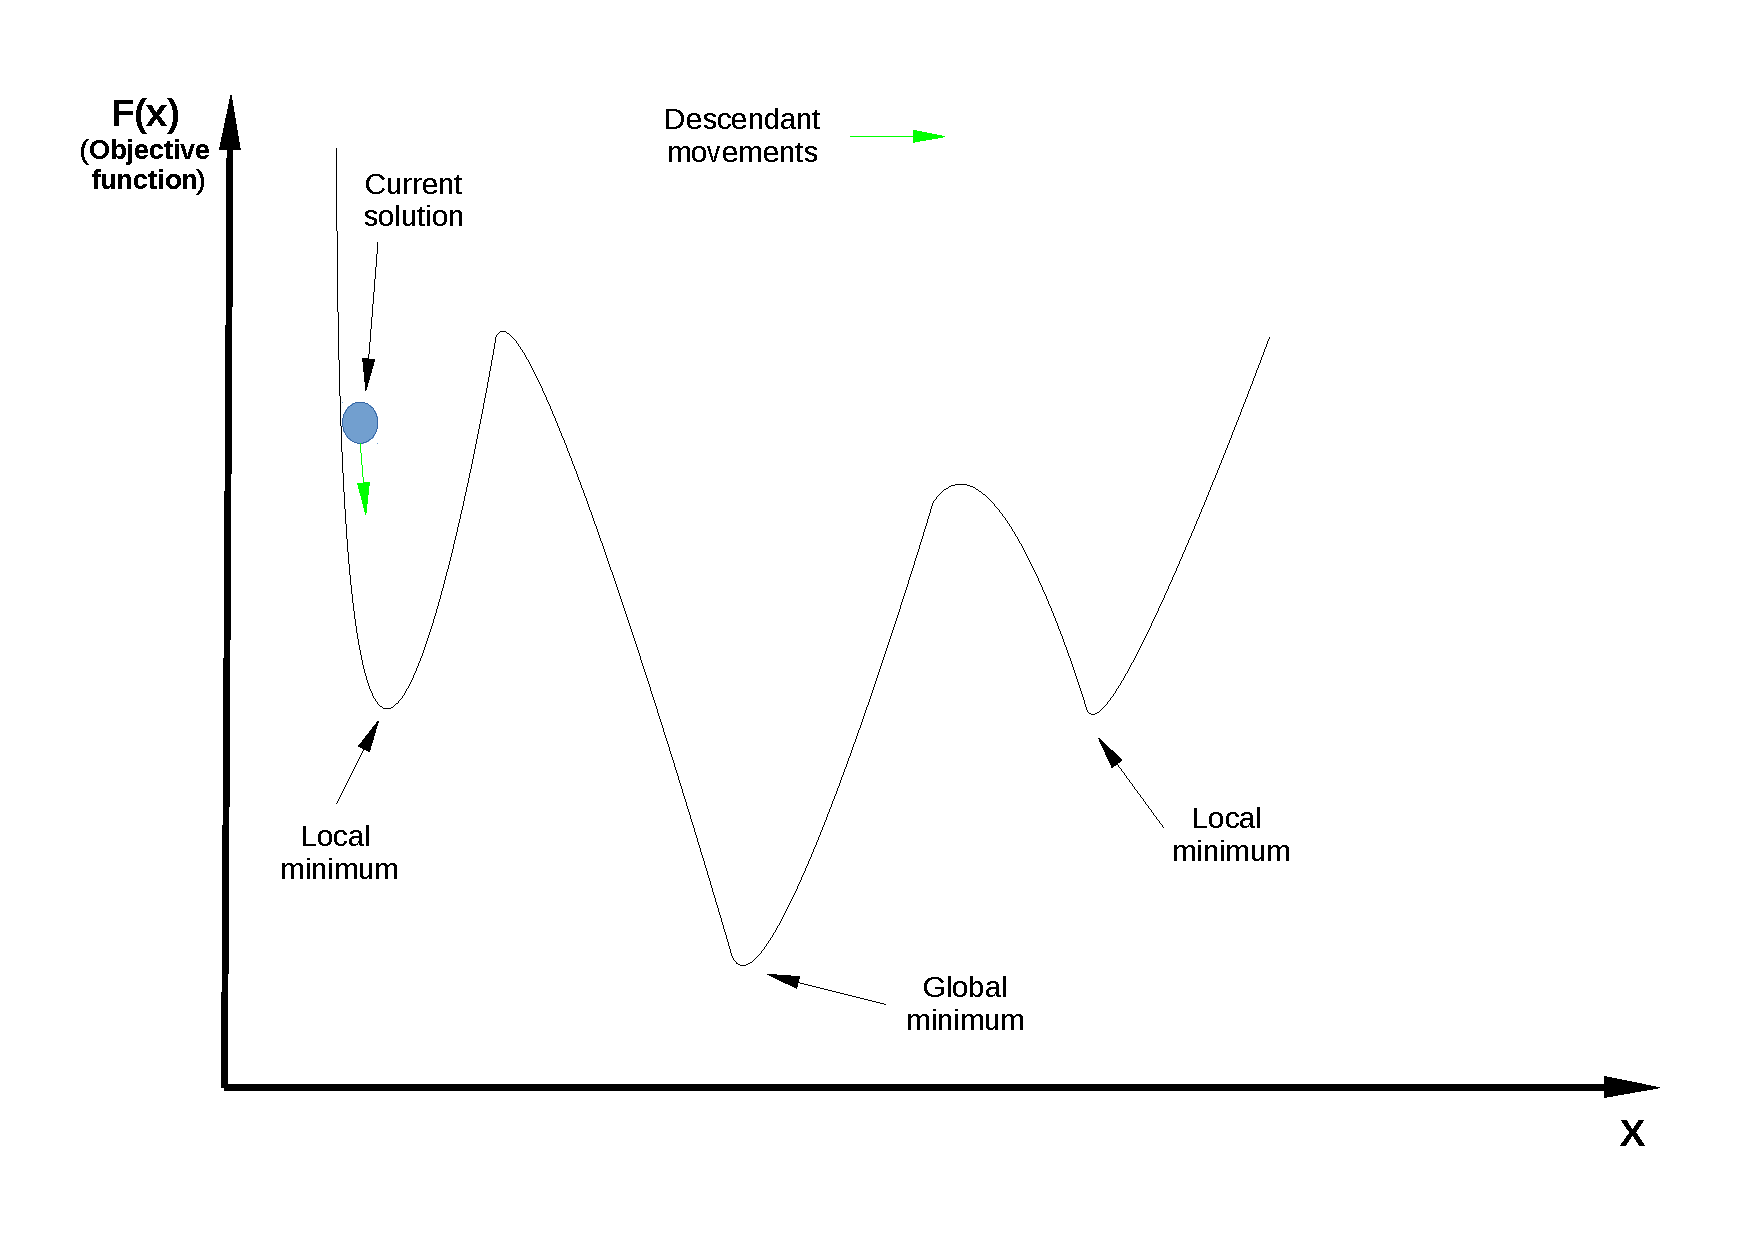
\includegraphics[width=\columnwidth,clip]{./Figs/IterativeSearchAlgorithm}\vspace{-0.5cm}
          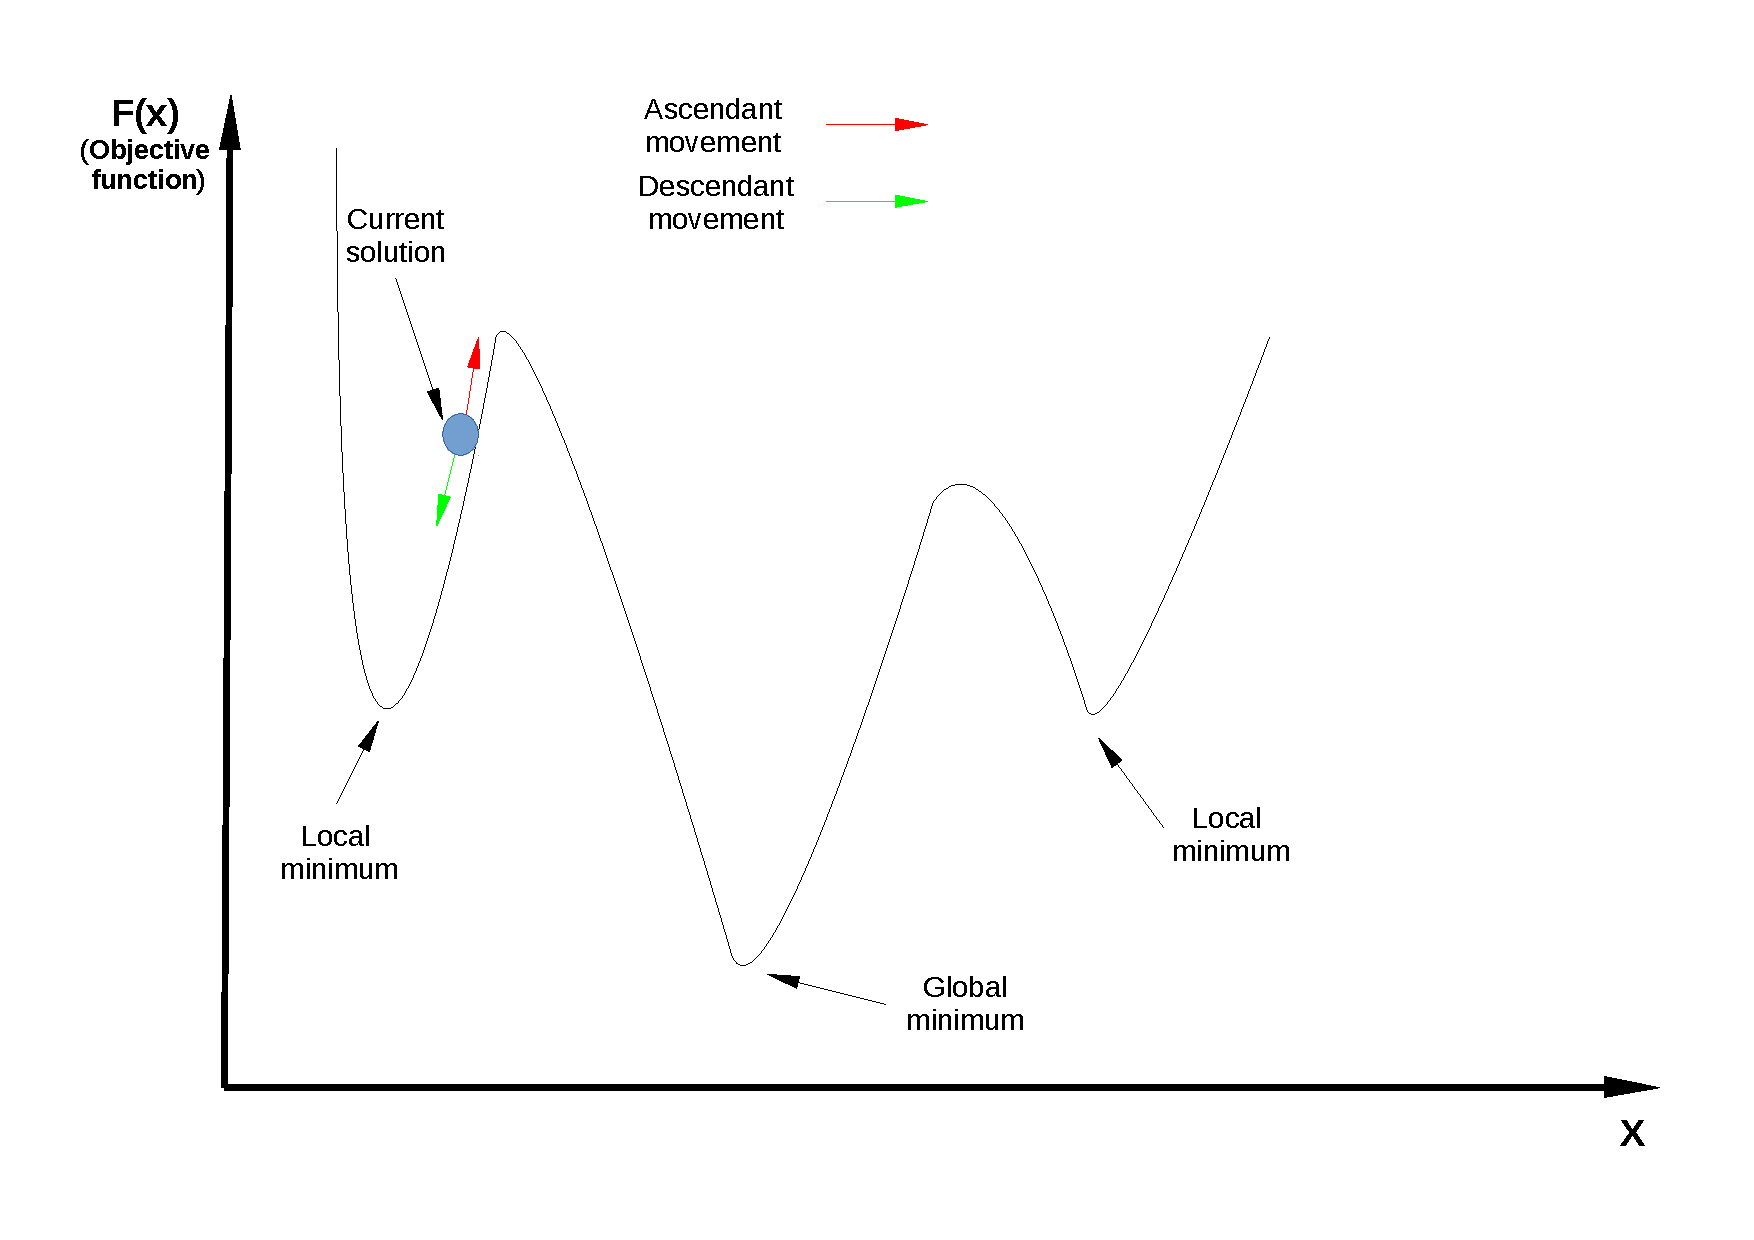
\includegraphics[width=\columnwidth,clip]{./Figs/SimulatedAnnealingAlgorithm}\vspace{-0.5cm}
           \caption{Graphical representation of iterative search (top) and the simulated annealing algorithms.} 
        %\end{center}%
\label{Chapter:GlobalOpt:Fig:IterativeSearch_SA_Algorithms}
\end{figure}
%%% Figure
\index{Optimisation!Iterative search algorithm}
In traditional iterative search methods (Algorithm~\ref{Chapter:GlobalOpt:Algorithm:IterativeSearch}), the function $F$ is continuously evaluated based on an initial estimate and if there is a decrease on the value of the function, then the point is accepted, otherwise it is rejected. This family of algorithms has two main issues: (a) the algorithm can remain in regions of local minima (Fig.~\ref{Chapter:GlobalOpt:Fig:IterativeSearch_SA_Algorithms}, top) and, (b) the solution will {\it always} depend on the initial estimate. Therefore, in order to find the global minima, iterative search algorithms need to be applied continuously starting from each local minima found.
\medskip

%%%
%%% ALGORITHM
%%%
\begin{algorithm}[h]%\scriptsize
   \SetKwData{Left}{left}\SetKwData{This}{this}\SetKwData{Up}{up}
   \SetKwFunction{Union}{Union}\SetKwFunction{FindCompress}{FindCompress}
   \SetKwInOut{Input}{Input}\SetKwInOut{Output}{Output}\SetKwInOut{Calculate}{Calculate}\SetKwInOut{Set}{Set}\SetKwInOut{Adjust}{Adjust}\SetKwInOut{Generate}{Generate}

      \Input{Given an initial estimative $x_{i}\in\Omega\subseteq\mathcal{R}^{n}$;}
      \While{ Convergence $\left(F\left(x_{v}\right)\le F\left(x_{i}\right)\right)$ }{ 
             \Generate{ A set of coordinate solutions $x_{v}$ based on $x_{i}$;}
              \Calculate{$\delta=F\left(x_{v}\right)-F\left(x_{i}\right)$}
              \If{$\delta \le 0$}{
                   $x_{i}=x_{v}$}}

 \caption{Iterative search algorithm.}\label{Chapter:GlobalOpt:Algorithm:IterativeSearch}
\end{algorithm}

The \SAA, as a typical local search algorithm~\citep{Tsallis_1996,Dekkers_1991}, is able to accept solution cordinates that do not lead to increase of the objective function. Thus it is able to `jump' regions of local minima in its continuous search to the global minima (Fig.~\ref{Chapter:GlobalOpt:Fig:IterativeSearch_SA_Algorithms}, bottom). The acceptance of points that leads to the increase of the objective function, $F\left(x_{k+1}\right) > F\left(x_{k}\right)$, is controlled by a stochastic submodel.


%%% Section
\subsection{Method Initialisation}\label{Chapter:GlobalOpt:Section:SAA}\index{Simulated annealing algorithm}\index{Optimisation!Simulated annealing algorithm}
Algorithm~\ref{Chapter:GlobalOpt:Algorithm:SAA} shows a simplified description of the \SAA as introduced by \citet{Corana_1987}\citep[see also][]{Goffe_1994}. The first step is to calculate the value of the objective function, $F\left(\mfr[\underline{X}]{}{0}\right)$ based on the initial vector of independent variables $\mfr[\underline{X}]{}{0}\subseteq\mathcal{R}^{n}$ and the temperature parameter\footnote{In the \SAA, temperature is a parameter in the algorithm and \underline{is not} related to the physical temperature.}, $T(t=0)=T_{0}$. A new solution-coordinate vector, $\mfr[\underline{X}]{}{1}$, is stochastically generated based on the previous iteration, $\mfr[\underline{X}]{}{0}$ and the new objective function, $F\left(\mfr[\underline{X}]{}{1}\right)$, is obtained. If the value of the function after the new iteration is smaller than the previous, $F\left(\mfr[\underline{X}]{}{1}\right) \le F\left(\mfr[\underline{X}]{}{0}\right)$, then the solution-coordinate is accepted $\left(\mfr[\underline{X}]{}{\text{opt}}=\mfr[\underline{X}]{}{\text{1}}\right)$, otherwise the {\it Metropolis criteria} is used.

%%% Section
\subsection{Metropolis Criteria}
\citet{Metropolis_1953}\index{Simulated annealing algorithm!Metropolis criteria} developed an algorithm to simulate the behaviour of an ensemble of atoms in equilibrium at a given temperature. At each stage of this algorithm, the position of every atom is represented by random movements that lead to energy gradient, $\Delta E$. The system is assumed stable when the energy of the system is the minimum. Therefore if $\Delta E \le 0$ the movement is accept, however if $\Delta E > 0$ the probability that the ensemble of atoms configuration be accepted is assessed by the following probability distribution function,
\begin{equation}
  \mathcal{P}\left(\Delta E\right) = \exp{\left[-\frc{\Delta E}{k_{B}T}\right]}, 
\end{equation}
where $k_{B}$ is the Boltzmann constant. A random number in the interval $[0,1]$ is selected $\left(\mathcal{N}_{r}\right)$ and if $\mathcal{P}\left(\Delta E\right) < \mathcal{N}_{r}$ the configuration is accepted. This acceptance criteria is based on the Boltzmann statistical distribution, and the continuous use of this criteria simulates the atom movement in thermal bath at temperature. 

%%% Section
\subsection{Analogy with Physical Annealing}
Thus, if the energy variation and  the ensemble of atoms configuration are represented by the objective function, $F\left(\underline{X}\right)$, and the vector of independent variables, $\underline{X}$, respectively, then the procedure adopted by \citet{Metropolis_1953} generates an ensemble of configurations for the optimisation problem at a given temperature $T$. In the analogy of the physical annealing process, the system is initially at melting temperature. The temperature is slowly reduced (\ie in stages) until the atoms reach an stable arrangement configuration (\ie low temperature). 
%%% Figure
\begin{figure}[h]
       % \begin{center}
          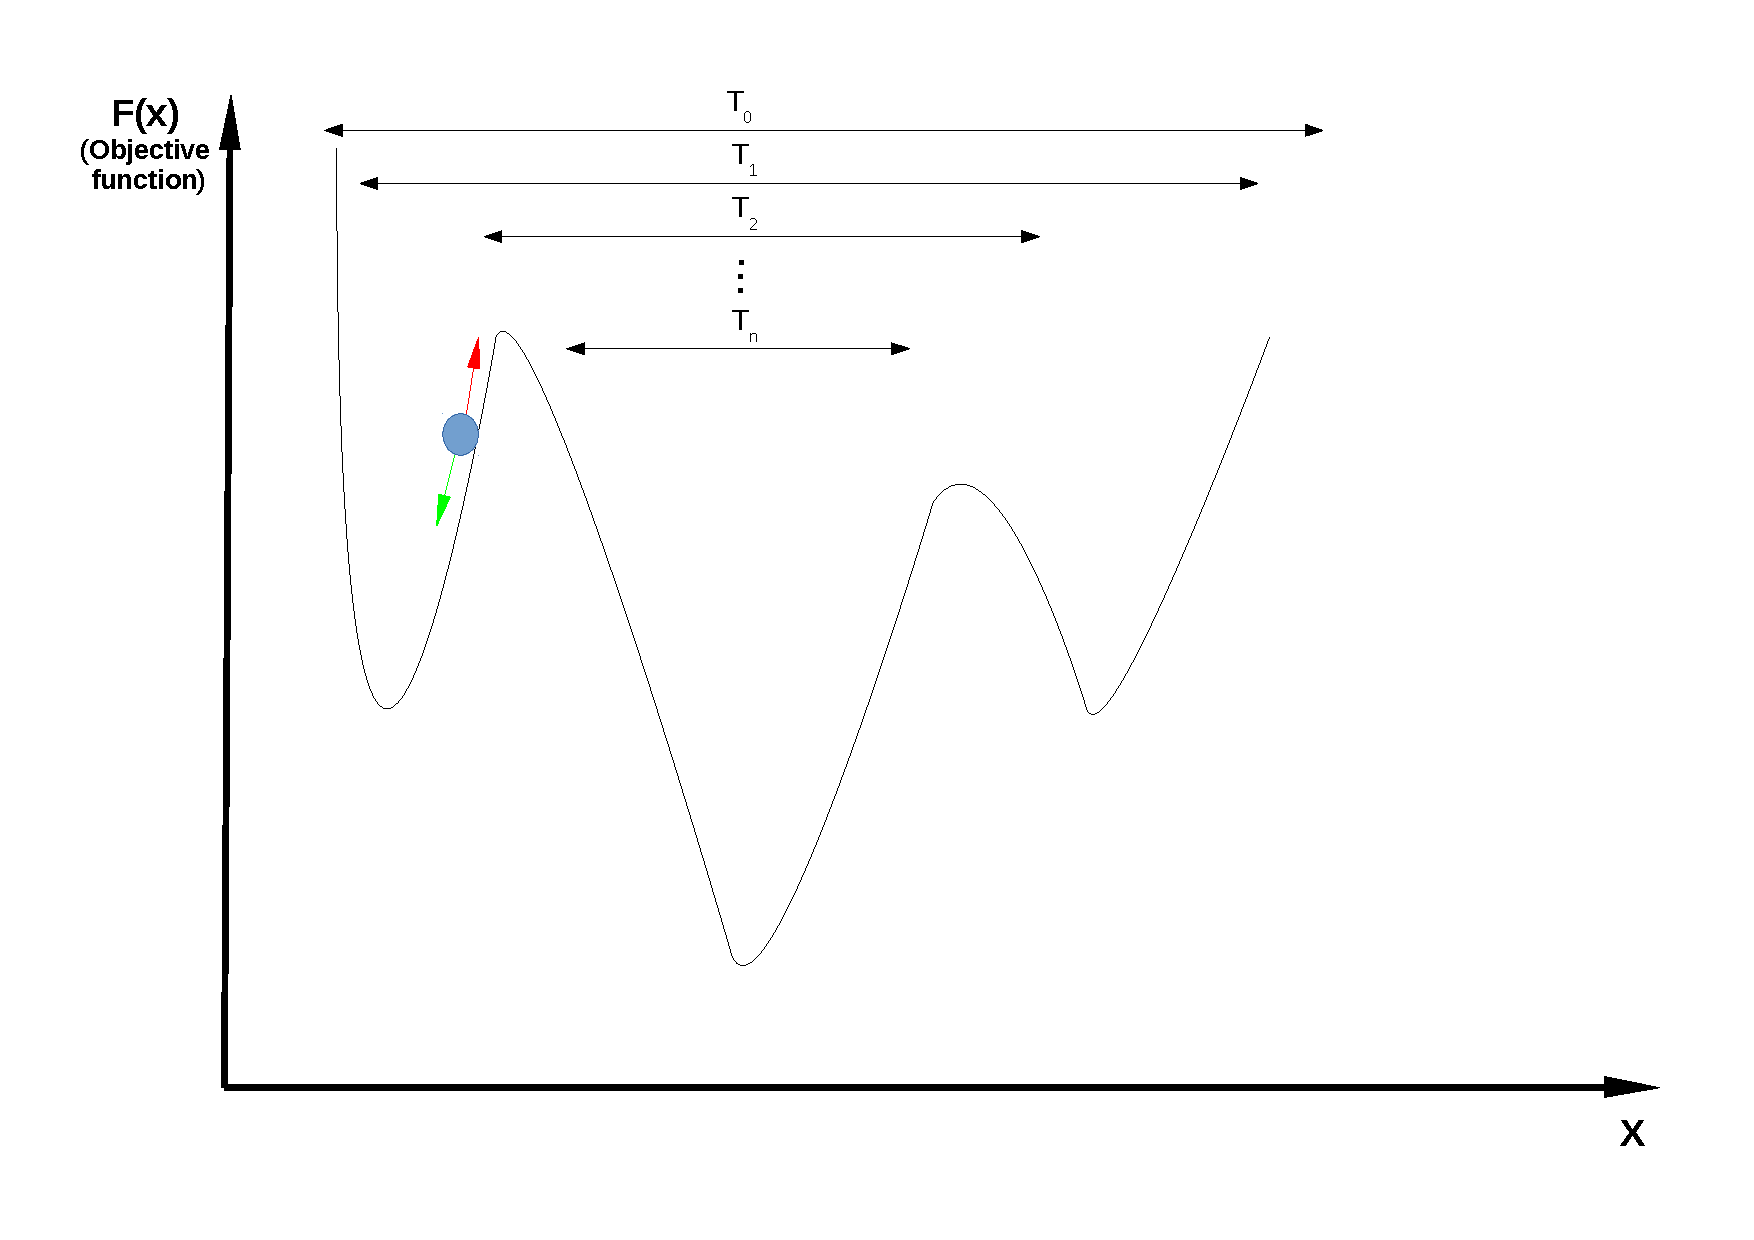
\includegraphics[width=\columnwidth,clip]{./Figs/SimulatedAnnealingAlgorithmTemperature}
           \caption{Graphical representation of the SAA's throughout the domain with smooth decrease of the temperature parameter.} 
        %\end{center}%
\label{Chapter:GlobalOpt:Fig:SimulatedAnnealingAlgorithmTemperature}
\end{figure}
%%% Figure
The implementation of the \SAA depends on a relatively large number of parameters, often called {\it cooling schedule} \citep[see][for a good review]{Nourani_1998}. During the \SAA simulation as the indices are incremented the temperature is reduced. It is important to notice that the larger the temperature, the larger the probability that the new configuration to be accepted. Overall, the \SAA scan throughout the domain with large acceptance of solution-coordinates, where the ascendant movements are required. As the temperature is reduced, the algorithm starts to accepts fewer new solution-coordinates, Fig.~\ref{Chapter:GlobalOpt:Fig:SimulatedAnnealingAlgorithmTemperature}. Thus, during the global optimisation the probability of acceptance of a new solution-coordinate that lead to an increase in the objective function tends asymptotically to zero due to the Boltzmann (or canonical) probability distribution function \citep{Tsallis_1996,Dekkers_1991}.


%%% Section
\subsection{Summary Description of the \SAA}
Model description in this section is a summary of the \SAA originally developed by \citet{Corana_1987} and \citet{Gomes_MSc_1999} and optimised by \citet{Goffe_1994} \citep[see also][]{gomes_2001}. Given a vector of solution-coordinate $\underline{X}\subseteq\mathcal{R}^{n}$ and the objective function $F\left(\underline{X}\right)$ that must be minimised. Algorithm~\ref{Chapter:GlobalOpt:Algorithm:SAA} can be divided into 10 main steps summarised in Fig.~\ref{Chapter:GlobalOpt:Fig:FlowChart}:
%%%
%%% ALGORITHM
%%%
\begin{algorithm}[h]%\scriptsize
   \SetKwData{Left}{left}\SetKwData{This}{this}\SetKwData{Up}{up}
   \SetKwFunction{Union}{Union}\SetKwFunction{FindCompress}{FindCompress}
   \SetKwInOut{Input}{Input}\SetKwInOut{Output}{Output}\SetKwInOut{Calculate}{Calculate}\SetKwInOut{Set}{Set}\SetKwInOut{Adjust}{Adjust}

      \Input{Given an initial estimative of the array of unknowns $\underline{X}$ and the cooling schedule list:}
      \Calculate{$F\left[\underline{X}^{\left(0\right)}\right]$}
      \Set{ $\underline{X}^{\left(\text{opt}\right)} = \underline{X}^{\left(0\right)}$ and $F\left[\underline{X}^{\left(\text{opt}\right)}\right] = F\left[\underline{X}^{\left(0\right)}\right]$ }

      \While{ Convergence }{ 
         \For{$l \leftarrow 1$ \KwTo$N_{T}$}{
             \For{$m \leftarrow 1$ \KwTo$N_{S}$}{
                 \For{$h \leftarrow 1$ \KwTo$N$}{
                     Update of array $\underline{X}$ \;
                 
                     \If{$\left[\underline{X}^{\left(i+1,h\right)}\ge\underline{a}\right.$ {\bf or} $\left.\underline{X}^{\left(i+1,h\right)}\le\underline{b}\right]$}{
                           \Calculate{$F\left[\underline{X}^{\left(i+1,h\right)}\right]$} 
                        }
                 
                     \eIf{$\left\{F\left[\underline{X}^{\left(i+1,h\right)}\right] > F\left[\underline{X}^{\left(i,h\right)}\right]\right\}$}{
                           \If{ (Metropolis criteria is accepted) }{
                                $\underline{X}^{(i,h)} = \underline{X}^{(i+1,h)}$\;
                                $F\left[\underline{X}^{(i,h)}\right] = F\left[\underline{X}^{(i+1,h)}\right]$      
                              }
                         }    {
                                $\underline{X}^{(i,h)} = \underline{X}^{(i+1,h)}$
                              }
                 
                     \If{ $F\left[\underline{X}^{(i+1,h)}\right] < F\left[\underline{X}^{(\text{opt})}\right]$ }{
                                $\underline{X}^{(\text{opt})} = \underline{X}^{(i+1,h)}$\;
                                $F\left[\underline{X}^{(\text{opt})}\right] = F\left[\underline{X}^{(i+1,h)}\right]$    
                        }
%
                 } % Loop h
             } % Loop m
%
             \Adjust{ Step-size matrix}
%
         } % Loop l
%
         \eIf{ $\left|F\left[\underline{X}^{(i,h)}\right] - F\left[\underline{X}^{(i+1,h)}\right]\right| < \epsilon$ }{
               \Calculate{ $F\left[\underline{X}^{(\text{opt})}\right]$}
             }{
               \Adjust{ Temperature parameter }} 
     } % While 
 \caption{Simmulated Annealing Algorithm.}\label{Chapter:GlobalOpt:Algorithm:SAA}
\end{algorithm}
\begin{enumerate}[{\bf Step 1: }]
%%%%%%%
   \item\label{Step1} An initial estimate of the vector of solution-coordinate $mfr[\underline{X}]{}{0}$ and the upper and lower limits, $b$ and $a$, of the solution domain.  We also need to initialise the following elements of the {\it cooling schedule}:
   \begin{itemize}
      \item Stepping matrix: $\underline{\underline{V}}_{0}$;
      \item Temperature: $T_{0}$;
      \item Stoppage criteria: $\varepsilon$;
      \item Maximum number of successive reduction of the temperature parameter: $N_{T_{e}}$;
      \item Maximum number of cycles: $N_{S}$;
      \item Number of directions: $N_{h}$;
      \item Parameter for controlling the size of the stepping matrix: $C$;
      \item Maximum number of iteration before the temperature reduction: $N_{T}$;
      \item Parameter for temperature reduction: $r_{T}$.
   \end{itemize}
   It is also worthy establishing the indices used in Algorithm~\ref{Chapter:GlobalOpt:Algorithm:SAA} that are initialised as zero:
   \begin{itemize}
      \item $i$: points or iterations;
      \item $j$: cycles along the coordinates;
      \item $m$: adjusts in the stepping matrix;
      \item $k$: temperature;
      \item $h$: direction of the generated set of solution-coordinates.
   \end{itemize}

%%%%%%%
   \item\label{Step2} The initial vector of solution-coordinate should be bounded, i.e., $a <\mfr[\underline{X}]{}{0}< b$. If any component of $\mfr[\underline{X}]{}{0}$ is out of bounds then a new $\mfr[\underline{X}]{}{0}$ is generated.

%%%%%%%
   \item\label{Step3} Calculate the function $F\left(\mfr[\underline{X}]{}{0}\right)$ and set up:
       \begin{itemize}
           \item $\mfr[\underline{X}]{}{i} = \mfr[\underline{X}]{}{\text{opt}} = \mfr[\underline{X}]{}{0}$, where $\mfr[\underline{X}]{}{i}$ represents
                 \begin{displaymath}
                    \mfr[\underline{X}]{}{i} = \left(X_{1}\; X_{2}\; \cdots \; X_{n-1}\;  X_{n}\right)^{\text{T}},
                 \end{displaymath}
            at the {\it i}$^{th}$ iteration;
           \item $F\left(\mfr[\underline{X}]{}{0}\right) = F\left(\mfr[\underline{X}]{}{i}\right) = \mfr[F]{}{i} = \mfr[F]{}{\text{opt}}$. 
       \end{itemize}

%%%%%%%
   \item\label{Step4} Let the vector $\underline{X}\subseteq\mathcal{R}^{n}$ be compose by the {\it canonical basis} $\underline{e}$, \ie generated based on a set of linearly independent generalised eigenvectors,
   \begin{displaymath}
      \underline{e} = \left[
             \begin{pmatrix}1 \\ 0 \\ 0 \\ \vdots \\ 0 \\ 0 \end{pmatrix},
             \begin{pmatrix}0 \\ 1 \\ 0 \\ \vdots \\ 0 \\ 0 \end{pmatrix},
             \begin{pmatrix}0 \\ 0 \\ 1 \\ \vdots \\ 0 \\ 0 \end{pmatrix},
             \cdots,
             \begin{pmatrix}0 \\ 0 \\ 0 \\ \vdots \\ 1 \\ 0 \end{pmatrix},
             \begin{pmatrix}0 \\ 0 \\ 0 \\ \vdots \\ 0 \\ 1 \end{pmatrix}
      \right],
   \end{displaymath}
A new solution-coordinate vector, $\mfr[\underline{X}]{}{i+1}$, is generated based on $\mfr[\underline{X}]{}{i}$ along the direction $h$,
      \begin{equation}
         \mfr[\underline{X}]{}{i,h+1} = \mfr[\underline{X}]{}{i,h} + R \mfr[\underline{\underline{V}}]{}{j}\mfr[\underline{e}]{}{h},\label{Chapter:GlobalOpt:Eqn:XEvolution}
      \end{equation}
where $\mfr[\underline{e}]{}{h}$ is the unity vector of the $h^{\text{th}}$ direction coordinate, $\mfr[\underline{\underline{V}}]{}{j}$ is the diagonal stepping matrix and $R$ is a number generated randomly in the $[-1,1]$ interval. Table~\ref{Chapter:GlobalOpt:Table:XEvolution} and Fig.~\ref{Chapter:GlobalOpt:Fig:SimulatedAnnealingAlgorithmOrthogonal} show how $\underline{X}$ is continuously generated in all directions, in which all movements are orthogonal to each other. Figure~\ref{Chapter:GlobalOpt:Fig:SimulatedAnnealingAlgorithmOrthogonal} shows an example of $\underline{X}$ generation for a function $F\left(X_{1},X_{2}\right)$ in $\mathcal{R}^{2}$, where the dot lines represent solution-coordinates that were not accepted by the {\it Metropolis Criteria}.

%%%%%%%
   \item\label{Step5} If the $h^{\text{th}}$ coordinate of $\mfr[\underline{X}]{}{i+1}$ lies out of bounds, \ie $\mfr[\underline{X}]{}{i+1} < a$ or $\mfr[\underline{X}]{}{i+1} > b$, then the algorithm returns to Step~\ref{Step4}.

%%%%%%%
   \item\label{Step6} Calculate $F\left(\mfr[\underline{X}]{}{i+1}\right) = \mfr[F]{}{i+1}$ and
       \begin{itemize}
           \item If $\mfr[F]{}{i+1}\le \mfr[F]{}{i}\;\Longrightarrow$: the new vector, $\mfr[\underline{X}]{}{i+1}$,  is accepted. Additionally, index $i$ and counter $N_{h}$ are incremented. If $\mfr[F]{}{i+1} < \mfr[F]{}{\text{opt}}$ then $\mfr[\underline{X}]{}{\text{opt}} = \mfr[\underline{X}]{}{i+1}$ and $\mfr[F]{}{\text{opt}} = \mfr[F]{}{i+1}$;
           \item Otherwise, the new vector {\bf\underline{may}} be rejected accordingly with the {\it Metropolis criteria},
               \begin{equation}
                   \mathcal{P} = \exp{\left[-\frc{\mfr[F]{}{i+1}-\mfr[F]{}{i}}{T_{k}}\right]}, \label{Chapter:GlobalOpt:Eqn:MetropolisCriteria}
               \end{equation}
$\mathcal{P}$ is compared against a random number $\mathcal{P}^{\star}$. If $\mathcal{P}^{\star}>\mathcal{P}$, the new vector is rejected , otherwise is accepted and the index $i$ and counter $N_{h}$ are incremented.
       \end{itemize}

%%%%%%%
   \item\label{Step7} Index $h$ is incremented and
       \begin{itemize}
           \item If $h<n$, then the algorithm returns to Step~\ref{Step4};
           \item Otherwise, $h=1$ and $j$ is incremented.
       \end{itemize}

%%%%%%%
   \item\label{Step8} Here,
       \begin{itemize}
           \item If $j<N_{s}$, then the algorithm returns to Step~\ref{Step4};
           \item Otherwise, the stepping matrix is incremented,
               \begin{subequations}
                  \begin{align}
                      & \mfr[\underline{\underline{V}}]{}{m+1} = \mfr[\underline{\underline{V}}]{}{m+1}\left[1 + \frc{5}{2}C\left(\frc{N_{a}}{N_{s}}-0.6\right)\right], \hspace{.5cm}\hfill \text{if }\frc{N_{a}}{N_{s}} > 0.6 \\
                      & \mfr[\underline{\underline{V}}]{}{m+1} = \mfr[\underline{\underline{V}}]{}{m+1}\left[1 + \frc{5}{2}C\left(0.4 - \frc{N_{a}}{N_{s}}\right)\right], \hspace{.5cm}\hfill \text{if }\frc{N_{a}}{N_{s}} < 0.4 \\ 
                      & \mfr[\underline{\underline{V}}]{}{m+1} = \mfr[\underline{\underline{V}}]{}{m+1},
                  \end{align}
               \end{subequations}
where $N_{a}$ is the number of accepted points, and as this number increases $\underline{\underline{V}}$ also increases. For a given $T$, the ratio between accepted and rejected numbers tends to decrease. It is clear that the dimension of $\underline{\underline{V}}$ is smaller as the solution-coordinates reaches the optimum region. However, as $T$ increases, the dimension of $\underline{\underline{V}}$ tends to increase to ensure that the algorithm can `jump' regions of local minimum. Therefore, \citet{Zhang_1993, Dekkers_1991,Goffe_1994} suggested that the ratio between accepted and rejected points to be close to unity.
       \end{itemize}

%%%%%%%
   \item\label{Step9} Here, 
       \begin{itemize}
           \item If $m<N_{T}$, then the algorithm returns to Step~\ref{Step4};
           \item Otherwise, parameter $T_{k}$ is reduced,
               \begin{equation}
                   T_{k+1} = r_{T} T_{k}
               \end{equation}
               and $\mfr[F]{}{k+1}=\mfr[F]{}{i}$.
       \end{itemize}
       As the temperature parameter decreases, the acceptance of solution-coordinates that lead to larger values of the function is less favourable, leading to an increase of the number of rejected solution-coordinates and the stepping matrix is reduced. Thus, the value of the function obtained at the new temperature is assumed optimum. 

%%%%%%%
   \item\label{Step10} Stoppage Criteria
       \begin{itemize}
           \item If $\left\|\mfr[F]{}{k}-\mfr[F]{}{\text{opt}}\right\|\le\epsilon$, the algorithm returns the numerical values;
           \item Otherwise, index $i$ is incremented, $\mfr[X]{}{i}=\mfr[X]{}{\text{opt}}$, $\mfr[F]{}{i}=\mfr[F]{}{\text{opt}}$ and the algorithm returns to Step~\ref{Step4}.
       \end{itemize}

%%%%%%%
\end{enumerate}


\begin{table}[h]
     Here we show the generation of solution-coordinate vector $\underline{X}$ at each direction. Consider $\underline{X}\subset\mathcal{R}^{n}$,
   \begin{displaymath}
        \begin{pmatrix}X_{1} \\ X_{2} \\ X_{3} \\ \vdots \\ X_{n-1} \\ X_{n} \end{pmatrix},
   \end{displaymath}
the stepping diagonal matrix, $\underline{\underline{V}}$,
   \begin{displaymath}
       \begin{pmatrix}
        V_{1,1} & 0      & 0      & \cdots & 0         & 0      \\
        0      & V_{2,2} & 0      & \cdots & 0         & 0      \\
        0      & 0      & V_{3,3} & \cdots & 0         & 0      \\
       \vdots  & \vdots & \vdots & \cdots & \vdots    & \vdots \\
        0      & 0      & 0      & \cdots & V_{n-1,n-1} & 0       \\
        0      & 0      & 0      & \cdots & 0         & V_{n,n} 
       \end{pmatrix},
   \end{displaymath}
and finally the unit vectors,
   \begin{displaymath}
      \underline{e} = \left[
             \begin{pmatrix}e_{1} \\ 0    \\ 0    \\ \vdots \\ 0     \\ 0    \end{pmatrix},
             \begin{pmatrix}0    \\ e_{2} \\ 0    \\ \vdots \\ 0     \\ 0    \end{pmatrix},
             \begin{pmatrix}0    \\ 0    \\ e_{3} \\ \vdots \\ 0     \\ 0    \end{pmatrix},
             \cdots,
             \begin{pmatrix}0    \\ 0    \\ 0    \\ \vdots \\ e_{n-1} \\ 0    \end{pmatrix},
             \begin{pmatrix}0    \\ 0    \\ 0    \\ \vdots \\ 0      \\ e_{n} \end{pmatrix}
      \right].
   \end{displaymath}
$\underline{X}$ varies in each spatial direction,
   \begin{eqnarray}
        \mfr[\underline{X}]{}{1}   &=& \mfr[\underline{X}]{}{0}   + R \underline{\underline{V}}\;\mfr[\underline{e}]{}{1}   \nonumber \\
        \mfr[\underline{X}]{}{2}   &=& \mfr[\underline{X}]{}{1}   + R \underline{\underline{V}}\;\mfr[\underline{e}]{}{2}   \nonumber \\
        \mfr[\underline{X}]{}{3}   &=& \mfr[\underline{X}]{}{2}   + R \underline{\underline{V}}\;\mfr[\underline{e}]{}{3}   \nonumber \\
                                   & &   \hspace{.5cm}\vdots                                                                \nonumber \\
        \mfr[\underline{X}]{}{h-1} &=& \mfr[\underline{X}]{}{h-2} + R \underline{\underline{V}}\;\mfr[\underline{e}]{}{h-1} \nonumber \\
        \mfr[\underline{X}]{}{h}   &=& \mfr[\underline{X}]{}{h-1} + R \underline{\underline{V}}\;\mfr[\underline{e}]{}{h}   \nonumber 
   \end{eqnarray}
Therefore, with a rigorous notation we recover Eqn.~\ref{Chapter:GlobalOpt:Eqn:XEvolution},
      \begin{displaymath}
         \mfr[\underline{X}]{}{i,h+1} = \mfr[\underline{X}]{}{i,h} + R \mfr[\underline{\underline{V}}]{}{j}\mfr[\underline{e}]{}{h}.
      \end{displaymath}

   \caption{Generation of the solution-coordinate vector $\underline{X}$.}\label{Chapter:GlobalOpt:Table:XEvolution},
\end{table}

%%% Figure
\begin{figure}[h]
       % \begin{center}
          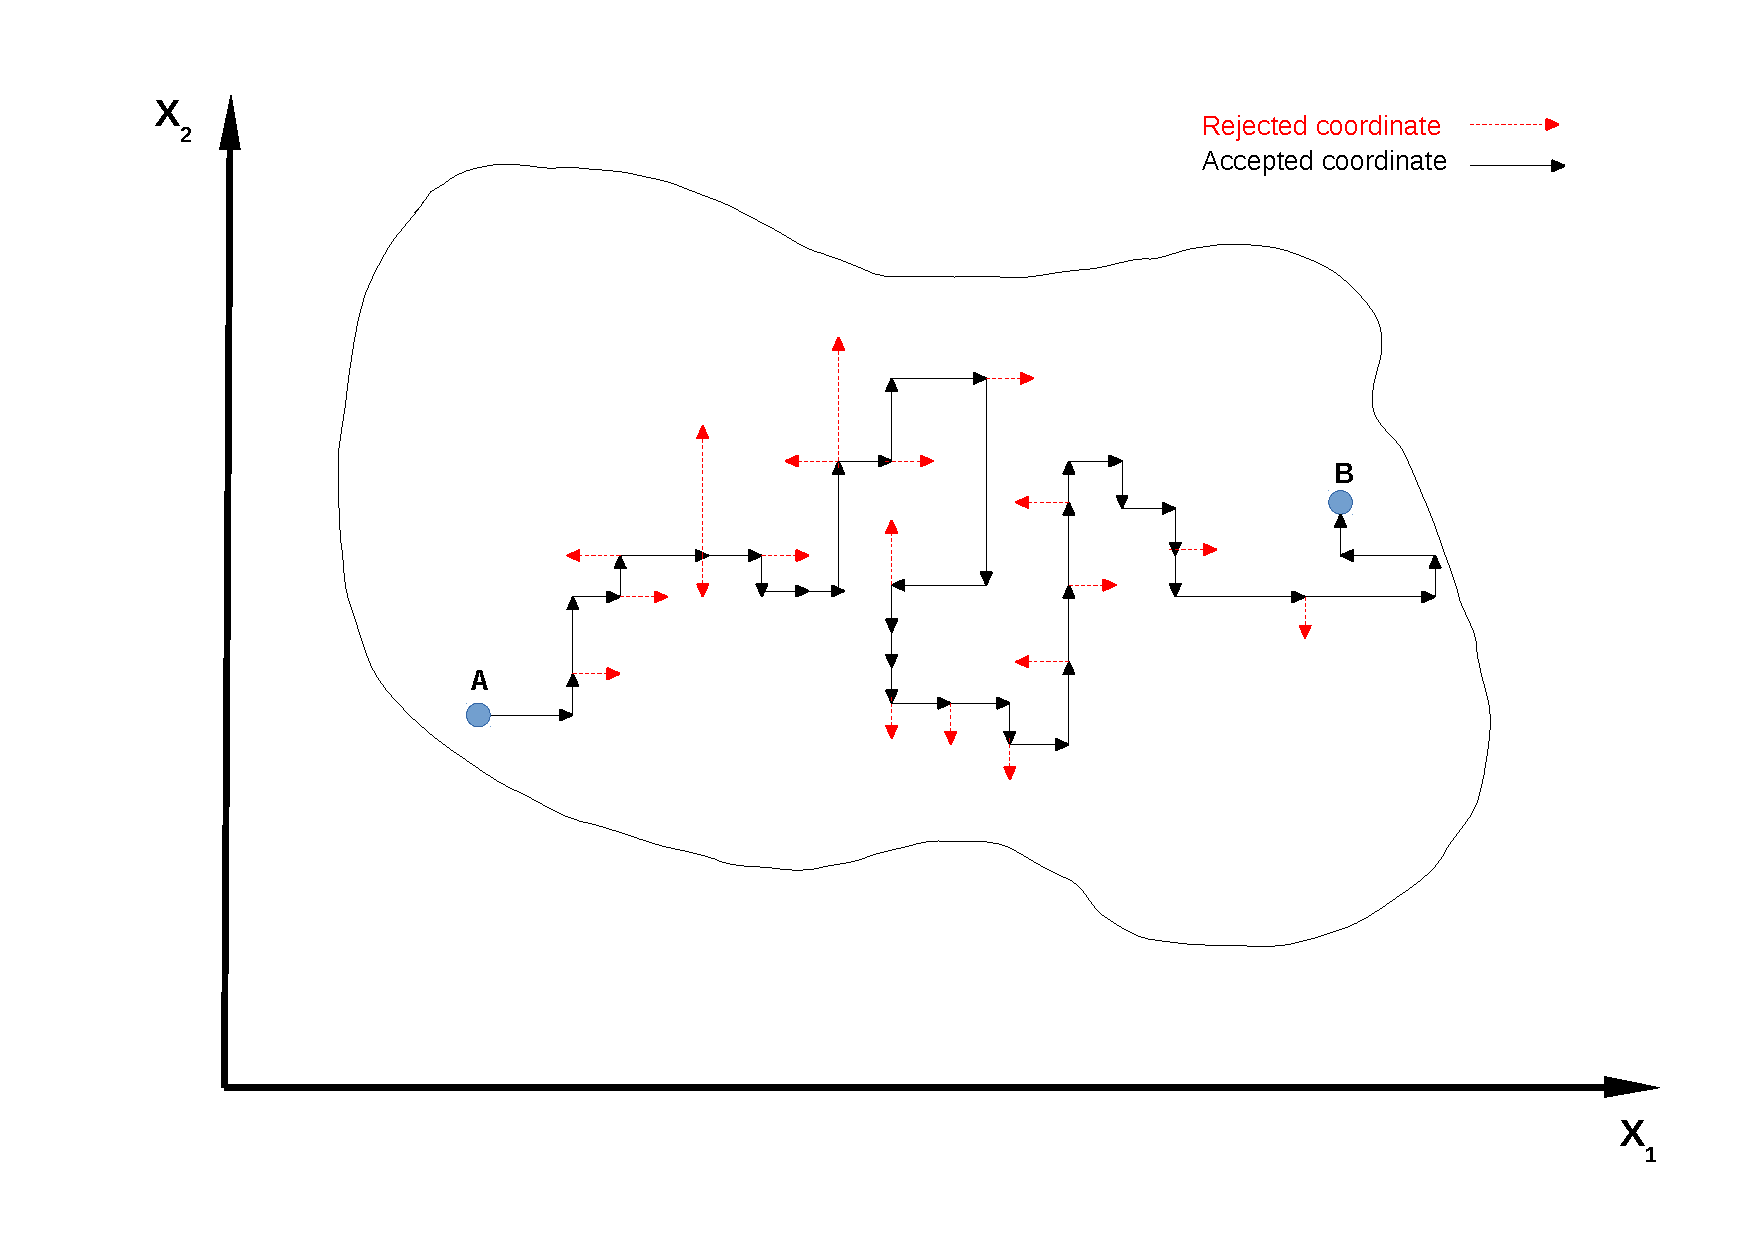
\includegraphics[width=\columnwidth,clip]{./Figs/SimulatedAnnealingAlgorithmOrthogonal}
           \caption{Graphical representation of the $\underline{X}\subseteq\mathcal{R}^{2}$ generation in different directions from initial solution-coordinate $A$ to final solution-coordinate $B$. Note that its evolution occurs through orthogonal movements.} 
        %\end{center}%
\label{Chapter:GlobalOpt:Fig:SimulatedAnnealingAlgorithmOrthogonal}
\end{figure}


\begin{figure}

% Define block styles
\tikzstyle{decision} =   [diamond,   draw, fill=blue!20, text width=4em, text badly centered, node distance=3cm, inner sep=2pt]
\tikzstyle{block} =      [rectangle, draw, fill=blue!20, text width=5em,   text centered,       rounded corners,   minimum height=4em]
\tikzstyle{blocklarge} = [rectangle, draw, fill=blue!20, text width=10em,  text centered,       rounded corners,   minimum height=4em]
\tikzstyle{blocklarge2} = [rectangle, draw, fill=blue!20, text width=15em,  text centered,       rounded corners,   minimum height=4em]
\tikzstyle{blockhuge} =  [rectangle, draw, fill=blue!20, text width=30em,  text centered,       rounded corners,   minimum height=4em]
\tikzstyle{line} =       [draw, -latex']
\tikzstyle{cloud} =      [draw, ellipse,   fill=red!20,  node distance=3cm,                                        minimum height=2em]
   
\begin{center} 
\begin{tikzpicture}[node distance = 3cm, auto]
    % Place nodes
    \node [blocklarge](init) {Initialisation of parameters.};
    \node [blockhuge, below of=init](procedure) {Execute a cycle of random movements in all directions. Accept or reject each solution-coordinate according to the {\it Metropolis criteria}. Store the optimum solution-coordinate.};

    \node [decision, below of=procedure] (decide1) {Number of cycles $> N_{s}$};

    \node [blocklarge2, below of=decide1](Stepping) {Adjust $\underline{\underline{V}}$. Re-initialise the number of cycles.};

    \node [decision, below of=Stepping] (decide2) {Number of stepping $> N_{T}$};
    \node [blockhuge, below of=decide2] (procedure2) {Reduce the temperature parameter. Re-initialise the number of adjusts. Select the current coordinate as optimum.};
    \node [decision, below of=procedure2] (Stoppage) {Is stoppage criteria met?}; 
    \node [block, below of=Stoppage, node distance=3cm] (stop) {Stop};

    % Draw edges
    \path [line] (init) -- (procedure);
    \path [line] (procedure) -- (decide1);
    \path [line] (decide1) -| node [near start] {no}  (procedure.east);
    \path [line] (decide1) -- node {yes} (Stepping);
    \path [line] (Stepping) -- (decide2);
    \path [line] (decide2) -| node [near start] {no} (procedure.east);
    \path [line] (decide2) -- node {yes} (procedure2);
    \path [line] (procedure2) -- (Stoppage);
    \path [line] (Stoppage) -| node [near start] {no} (procedure.east);
    \path [line] (Stoppage) -- node {yes} (stop);

\end{tikzpicture}
\end{center}
\caption{Flowchart of the \SAA.}
\label{Chapter:GlobalOpt:Fig:FlowChart}
\end{figure}

%%% Section
\subsection{Applying the \SAA in the VLE Problem}
For the optimisation problem described in Algorithm~\ref{VLE_Problem:Algorithm}, the objective function is the molar Gibbs free energy, \ie $F\left(\underline{X}\right) = g\left(\mfr[x]{1}{L},\cdots,\mfr[x]{n_{c}-1}{L},L\right)$,  and the vector of solution-coordinates is,
     \begin{displaymath}
          \underline{X} = 
                 \begin{pmatrix}\mfr[x]{1}{L} \\ \mfr[x]{2}{L} \\  \mfr[x]{3}{L} \\ \vdots \\  \mfr[x]{n_{c}-1}{L} \\ L \end{pmatrix},
     \end{displaymath}
with the following linear constraints,
     \begin{displaymath}
           0 < L < 1, \hspace{1cm} 0 < \mfr[x]{i}{L} < 1,\;\left(\forall i=1,\cdots,n_{c}-1\right), \text{ and } \hspace{1cm} \summation_{i=1}^{n_{c}-1}\mfr[x]{i}{L} < 1
     \end{displaymath}









%%%
%%% Section
%%%
\section{Particle Swarm Algorithm}

To be added.
